\documentclass[10pt,a4paper,english]{article}
\usepackage{geometry,metalogo,hyperref,babel,mdwlist,array,multicol}
\usepackage[default]{raleway}
\usepackage[scaled=1]{sourcecodepro}

\hypersetup{
    colorlinks,
    citecolor=blue,
    filecolor=blue,
    linkcolor=blue,
    urlcolor=blue
}
\newcommand*\file[1]{\href{run:#1.pdf}{#1}}

\title{\bfseries
	\Huge raleway\\
	\Large Matt McInerney’s Raleway family for \LaTeX
}

\author{Silke Hofstra, \href{mailto:tex@slxh.nl}{tex@slxh.nl}}
\date{Documentation for raleway v1.6.\\ \today}
\begin{document}
\maketitle
\begin{multicols}{2}
This package provides the Raleway family in an easy to use way. For \XeLaTeX\ and \LuaLaTeX\ users the original OpenType fonts are used. The entire font family is included.

The current raleway family is an extension of the original Raleway Thin by Matt McInerney. The family has been extended by Impallari, and is currently maintained by The League of Moveable Type. For more information see \href{https://www.theleagueofmoveabletype.com/raleway}{The League of Moveable Type website} or the \href{https://github.com/theleagueof/raleway}{Raleway GitHub repo}.

This package is also available on \href{https://github.com/silkeh/latex-raleway}{GitHub}.

\section{Options}
The package has the following options:
\begin{itemize*}
	\item \textbf{oldstyle, osf}:  use old style numbers.
	\item \textbf{lining, nf, lf}: use lining numbers.
%	\item \textbf{tabular}:        use fixed-width numbers.
%	\item \textbf{proportional}:   use normal numbers.
	\item \textbf{black}:          \texttt{\textbackslash bfseries} is black.
	\item \textbf{extrabold}:      \texttt{\textbackslash bfseries} is extrabold.
	\item \textbf{semibold}:       \texttt{\textbackslash bfseries} is semibold.
	\item \textbf{bold}:           \texttt{\textbackslash bfseries} is bold.
	\item \textbf{thin}:           \texttt{\textbackslash mdseries} is thin.
	\item \textbf{extralight}:     \texttt{\textbackslash mdseries} is extra light.
	\item \textbf{light}:          \texttt{\textbackslash mdseries} is light.
	\item \textbf{regular}:        \texttt{\textbackslash mdseries} is regular.
	\item \textbf{medium}:         \texttt{\textbackslash mdseries} is medium.
	\item \textbf{scale, scaled}:  Change the scaling with a factor. For example:  \texttt{scale=.5}
	\item \textbf{default}:        Raleway is set as the default font family and as the sans serif family.
	\item \textbf{nosfdefault}:    Raleway is not set as sans-serif family.
	\item \textbf{type1, t1}:      Override automatic detection and use the Type 1 fonts.
	\item \textbf{opentype, otf}:  Override automatic detection and use OpenType fonts.
\end{itemize*}
The following options are enabled by default: oldstyle, proportional, bold and regular.

\section{Commands}
Commands for all weights are also provided for \XeLaTeX\ and \LuaLaTeX\ users.
\begin{itemize*}
	\item \texttt{\bfseries \textbackslash raleway}
		-- the regular and bold weights.
	\item \texttt{\bfseries \textbackslash ralewaymedium}
		-- the medium and bold weights.
	\item \texttt{\bfseries \textbackslash ralewaylight}
		-- the light and semibold weights.
	\item \texttt{\bfseries \textbackslash ralewayextra}
		-- the extra light and extra bold weights.
	\item \texttt{\bfseries \textbackslash ralewaythin}
		-- the thin and black weights.
\end{itemize*}

\section{Licence}
The Raleway typeface is available under the \href{http://scripts.sil.org/OFL}{SIL Open Font License 1.1}.\\
All \LaTeX\ code is available under the \href{http://www.latex-project.org/lppl/}{\LaTeX\ project public license} v1.3 or later.

\section{Specimen}
Simple specimen are included on page \pageref{sec:specimen}.
As you can see the font currently has no italics.

\section{OpenType}
The OpenType fonts have many features, including old style numerals (1 6 9),  ligatures (ff fi fl) and stylistic alternatives ({\addfontfeature{Style=Alternate} l a g}).

\subsection{Features}
A complete list of available font features is available on page \pageref{sec:otfinfo}. More information on how to use font features can be found in the \href{http://mirror.ctan.org/macros/latex/contrib/fontspec/fontspec.pdf}{fontspec documentation}.

\subsection{Files}
\begin{itemize*}
	\item Raleway-Thin.otf
	\item Raleway-Thin-Italic.otf
	\item Raleway-ExtraLight.otf
	\item Raleway-ExtraLight-Italic.otf
	\item Raleway-Light.otf
	\item Raleway-Light-Italic.otf
	\item Raleway-Regular.otf
	\item Raleway-Regular-Italic.otf
	\item Raleway-Medium.otf
	\item Raleway-Medium-Italic.otf
	\item Raleway-Semibold.otf
	\item Raleway-Semibold-Italic.otf
	\item Raleway-Bold.otf
	\item Raleway-Bold-Italic.otf
	\item Raleway-ExtraBold.otf
	\item Raleway-Black-Italic.otf
	\item Raleway-Black.otf
	\item Raleway-Black-Italic.otf
\end{itemize*}

\section{Type1}
The following Type1 font families are included:
\begin{itemize*}
%	\item Raleway-LF
	\item Raleway-TLF
%	\item Raleway-OsF
	\item Raleway-TOsF
\end{itemize*}
With series ‘t’, ‘el’, ‘l’, ‘m’, ‘mb’, ‘sb’, ‘b’, ‘eb’, ‘k’ and shapes ‘n’ and ‘sc’, ‘it’ and ‘scit’.

\textbf{Please note:} to use italic smallcaps the \texttt{slantsc} package is required.

\section{Version history}
\subsection*{1.6}
\begin{itemize*}
\item Update to the The League of Moveable Type variant, version 4.101.
\end{itemize*}

\subsection*{1.5}
\begin{itemize*}
\item Fixed the \texttt{semibold} option.
\end{itemize*}

\subsection*{1.4}
\begin{itemize*}
	\item Johannes Choo: have sfdefault set ItalicFont and BoldItalicFont (Fixes \href{https://github.com/silkeh/latex-raleway/issues/1}{issue~\#1}).
\end{itemize*}

\subsection*{1.3}
\begin{itemize*}
	\item Fixed scaling issue.
\end{itemize*}

\subsection*{1.2}
\begin{itemize*}
	\item Fixed errors in weight implementation.
	\item Fonts updates to v3.0, which includes support for Cyrillic.
\end{itemize*}

\subsection*{1.1}
\begin{itemize*}
	\item Weights are now handled with the \href{http://www.ctan.org/pkg/mweights}{mweights} package.
	\item Fonts updated to v2.5, which includes italics.
\end{itemize*}

\subsection*{1.0}
\begin{itemize*}
	\item Initial release with v2.2 of the fonts.
\end{itemize*}

%\section{Known issues}

\vspace{0pt plus 1filll}\mbox{}
\newpage
\end{multicols}

\section{Specimen}
\label{sec:specimen}
\subsection{OpenType}
\begin{figure}[ht]
	\centering
	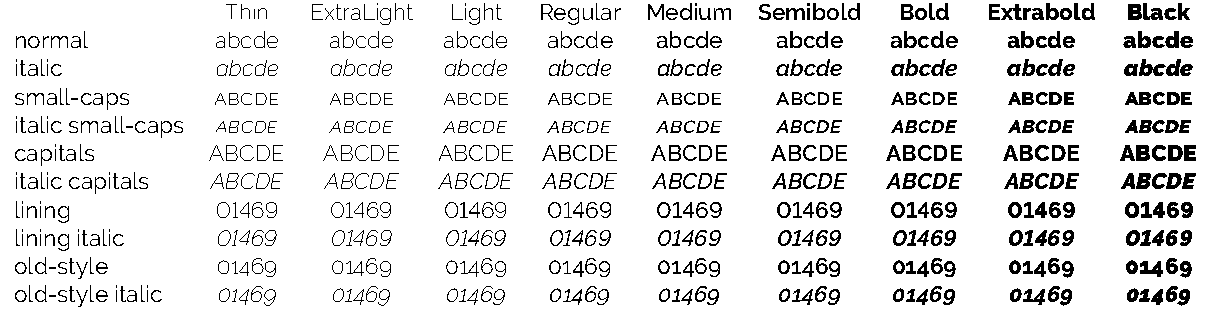
\includegraphics[width=\textwidth]{raleway-otf-specimen}
\end{figure}
This table can also be found in \file{raleway-otf-specimen}.

\subsection{Type1}
\begin{figure}[ht]
	\centering
	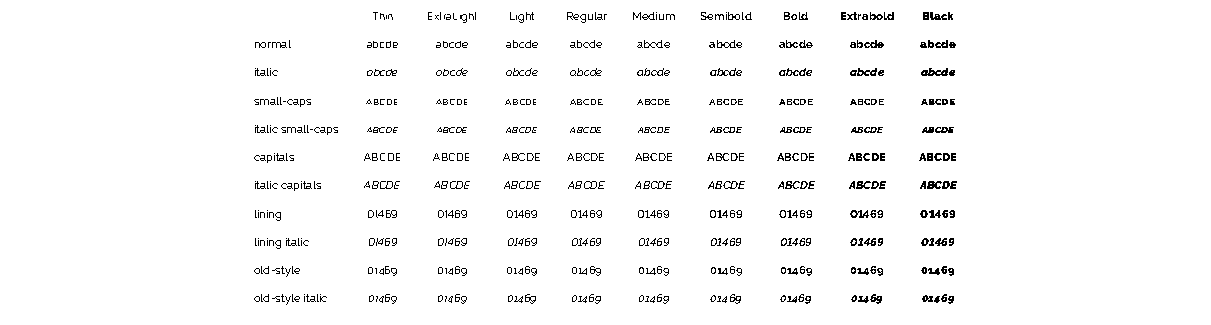
\includegraphics[width=\textwidth]{raleway-type1-specimen}
\end{figure}
This table can also be found in \file{raleway-type1-specimen}.

\newpage
\section{Opentype features}
\label{sec:otfinfo}

\begin{figure}[ht]
	\centering
	\begin{tabular}{>{\ttfamily}l l}
		aalt & Access All Alternates \\
		dlig & Discretionary Ligatures \\
		kern & Kerning \\
		liga & Standard Ligatures \\
		lnum & Lining Figures \\
		onum & Oldstyle Figures \\
		salt & Stylistic Alternates \\
		smcp & Small Capitals \\
		ss01 & Stylistic Set 1 \\
		ss02 & Stylistic Set 2 \\
	\end{tabular}
\end{figure}
(list generated with otfinfo)

\end{document}
